% Build: cd report && latexmk -xelatex report.tex
\documentclass[11pt,a4paper]{article}

% ---------- fill these in ----------
\newcommand{\studentname}{นายเมธัส ทองจันทร์}
\newcommand{\studentid}{6606022610030}
\newcommand{\appurl}{\url{https://miletae-bigbike.streamlit.app/}}
\newcommand{\repourl}{https://github.com/Shinnamon-Roll/nlpAssign2}
% -----------------------------------

\usepackage{fontspec}
\setmainfont{Sarabun}[Scale=1.05]
\newfontfamily\headfont{Chakra Petch}[BoldFont={Chakra Petch SemiBold}]
\XeTeXlinebreaklocale "th"
\XeTeXlinebreakskip = 0pt plus 1pt
\linespread{1.25}

\usepackage[margin=2.2cm]{geometry}
\usepackage{graphicx}
\usepackage{xcolor}
\usepackage{titlesec}
\usepackage{enumitem}
\usepackage{booktabs}
\usepackage{tabularx}
\usepackage{fancyhdr}
\usepackage[font=small,labelfont=bf]{caption}
\usepackage{float}
\usepackage[most]{tcolorbox}
\usepackage{tikz}
\usetikzlibrary{positioning,arrows.meta}
\usepackage[hidelinks]{hyperref}

\definecolor{ink}{HTML}{1B2733}
\definecolor{steel}{HTML}{5E6B78}
\definecolor{concrete}{HTML}{E6E8EB}
\definecolor{panel}{HTML}{F7F8F9}
\definecolor{tag}{HTML}{F2C230}
\definecolor{nf}{HTML}{B3362C}

\titleformat{\section}{\headfont\Large\bfseries\color{ink}}{\thesection}{0.6em}{}
\titleformat{\subsection}{\headfont\large\bfseries\color{ink}}{\thesubsection}{0.6em}{}
\renewcommand{\figurename}{ภาพที่}
\renewcommand{\tablename}{ตารางที่}
\setlist{itemsep=2pt,topsep=4pt}

\pagestyle{fancy}
\fancyhf{}
\lhead{\small\color{steel}พี่ไมล์ ผู้ช่วยเลือกบิ๊กไบค์ (RAG Chatbot)}
\rhead{\small\color{steel}\thepage}
\renewcommand{\headrulewidth}{0.4pt}

\newtcolorbox{note}{colback=panel,colframe=steel!40,boxrule=0.5pt,arc=2pt,left=8pt,right=8pt}
\newtcolorbox{promptbox}{colback=concrete,colframe=concrete,arc=2pt,left=8pt,right=8pt,fontupper=\small}

\newcommand{\shot}[3]{% file, width, caption
  \begin{figure}[H]\centering
  \fcolorbox{steel!40}{white}{\includegraphics[width=#2]{img/#1}}
  \caption{#3}\end{figure}}

\begin{document}

% ---------------- title ----------------
\begin{titlepage}
\begin{tcolorbox}[colback=ink,colframe=ink,arc=4pt,left=16pt,right=16pt,top=14pt,bottom=14pt]
{\color{white}\headfont\fontsize{30}{36}\selectfont ไมล์แท้ บิ๊กไบค์}\\[4pt]
{\color{white!85!ink}\large พี่ไมล์ ผู้ช่วย AI ตอบคำถามร้านบิ๊กไบค์มือสองด้วยเทคนิค RAG}
\end{tcolorbox}
\vspace{1.5cm}
{\headfont\Large แบบทดสอบเก็บคะแนนครั้งที่ 2: Web Application ระบบ RAG}\\[8pt]
รายงานภาพหน้าจอการทำงานของหน้าเว็บ พร้อมคำอธิบาย

\vspace{1.5cm}
\renewcommand{\arraystretch}{1.6}
\begin{tabularx}{\textwidth}{@{}lX@{}}
ชื่อ-สกุล & \studentname \\
รหัสนักศึกษา & \studentid \\
หัวข้อ & ผู้ช่วย AI ร้านขายรถบิ๊กไบค์มือสอง (ร้านสมมติ ``ไมล์แท้ บิ๊กไบค์'') \\
URL หน้าเว็บ & \appurl \\
GitHub & \url{\repourl} \\
\end{tabularx}

\vfill
\begin{note}\small
ร้าน ``ไมล์แท้ บิ๊กไบค์'' เป็นร้านสมมติที่สร้างขึ้นสำหรับเดโม รูปรถมาจาก dbigbike.com ซึ่งเป็นเว็บของผู้จัดทำและได้รับอนุญาตแล้ว
ราคา เลขไมล์ สภาพรถ นโยบายร้าน และข้อมูลติดต่อทั้งหมดเป็นข้อมูลจำลอง
\end{note}
\end{titlepage}

% ---------------- 1 ----------------
\section{ภาพรวมของระบบ}
ลูกค้าร้านรถมือสองมักถามคำถามซ้ำ ๆ เช่น ``MT-09 ยังอยู่ไหม ราคาเท่าไร'' ``งบไม่เกิน 3 แสนมีรุ่นไหนบ้าง'' หรือ ``ผ่อนดอกเบี้ยกี่เปอร์เซ็นต์''
พี่ไมล์ตอบคำถามเหล่านี้จากเอกสารของร้านเท่านั้น ทุกคำตอบแนบเอกสารอ้างอิงให้ตรวจสอบได้
และถ้าเอกสารไม่มีคำตอบ ระบบจะตอบว่า ``ไม่พบข้อมูลในเอกสาร'' แทนการเดา

\begin{itemize}
  \item \textbf{เทคโนโลยี:} Streamlit (หน้าเว็บ), sentence-transformers \texttt{intfloat/multilingual-e5-small} (embedding),
        FAISS (vector search), PyThaiNLP (ตัดประโยคภาษาไทย), Google Gemini ผ่าน SDK \texttt{google-genai} (LLM)
  \item \textbf{Deploy:} Streamlit Community Cloud อ่าน API key จาก \texttt{st.secrets["GEMINI\_API\_KEY"]} ไม่มี key อยู่ใน repository
\end{itemize}

\begin{figure}[H]\centering
\begin{tikzpicture}[
  box/.style={draw=steel,fill=panel,rounded corners=2pt,minimum height=9mm,text width=24mm,align=center,font=\small},
  hot/.style={box,fill=tag!60},
  arr/.style={-{Stealth[length=2.2mm]},color=ink,thick}]
\node[box] (load) {โหลด + ทำความสะอาด\\ \texttt{data/*.md}};
\node[box,right=6mm of load] (chunk) {Chunking\\ตามหัวข้อ + ความยาว};
\node[box,right=6mm of chunk] (embed) {Embedding\\e5-small (passage:)};
\node[box,right=6mm of embed] (faiss) {FAISS\\IndexFlatIP};
\node[box,below=12mm of faiss] (ret) {Retrieve top-5\\(query:)};
\node[box,left=6mm of ret] (prompt) {Prompt + Context\\+ ประวัติแชต};
\node[hot,left=6mm of prompt] (llm) {Gemini\\3.8 Flash};
\node[box,left=6mm of llm] (ui) {หน้าเว็บ Streamlit\\คำตอบ + อ้างอิง};
\draw[arr] (load)--(chunk); \draw[arr] (chunk)--(embed); \draw[arr] (embed)--(faiss);
\draw[arr] (faiss)--(ret); \draw[arr] (ret)--(prompt); \draw[arr] (prompt)--(llm); \draw[arr] (llm)--(ui);
\end{tikzpicture}
\caption{ขั้นตอนการทำงานของระบบ RAG ใน \texttt{rag.py} ส่วนแถวบนสร้างครั้งเดียวตอนเปิดแอป ส่วนแถวล่างทำทุกคำถาม}
\end{figure}

% ---------------- 2 ----------------
\section{เอกสารความรู้และคำถามทดสอบ}
\begin{table}[H]\centering\small
\begin{tabularx}{\textwidth}{@{}lX@{}}\toprule
ไฟล์ใน \texttt{data/} & เนื้อหา \\\midrule
\texttt{bike\_*.md} (44 ไฟล์) & รถ 1 คันต่อ 1 ไฟล์: รหัสสต็อก ราคา ส่วนลด เลขไมล์ สี เกรดสภาพ สถานะ สเปค ของแต่ง การรับประกัน ตัวอย่างค่างวด และ URL รูป \\
\texttt{inventory\_summary.md} & ตารางสรุปรถทั้ง 44 คัน ใช้ตอบคำถามเปรียบเทียบ กรองราคา และนับจำนวน \\
\texttt{shop\_*.md} (8 ไฟล์) & ข้อมูลร้าน รับประกัน ไฟแนนซ์ เทิร์นรถ โอนเล่ม จอง/ทดลองขับ ส่งรถ/บริการหลังการขาย และ FAQ \\
\texttt{guide\_*.md} (3 ไฟล์) & คู่มือเลือกบิ๊กไบค์มือสอง เลือกคันแรกตามงบ และการดูแลรถ \\
\texttt{bikes.csv} & ข้อมูลสต็อกหลัก ใช้สร้างไฟล์รถทุกไฟล์ด้วย \texttt{make\_data.py} \\\bottomrule
\end{tabularx}
\caption{เอกสารความรู้: 57 ไฟล์ รวม 143,928 ตัวอักษร (เกณฑ์คือ $\ge$ 10 ไฟล์ หรือ $\ge$ 15,000 ตัวอักษร)}
\end{table}

\texttt{test\_questions.csv} มีคำถาม 31 ข้อ แบ่งเป็นคำถามที่ตอบได้ 26 ข้อ และคำถามที่ไม่มีคำตอบในเอกสาร 5 ข้อ
คำถามที่ไม่มีคำตอบได้แก่ เช่ารถรายวัน ซ่อมรถยนต์ บริษัทประกันภัย สาขาต่างประเทศ และพยากรณ์อากาศ
ทุกข้อระบุคำตอบที่ถูกต้องและไฟล์ที่เป็นแหล่งที่มา

% ---------------- 3 ----------------
\section{เทคนิค RAG ที่ใช้}
\subsection{Document Loading \& Chunking}
\begin{itemize}
  \item อ่านไฟล์ Markdown ทุกไฟล์ แล้วแยกบรรทัด ``รูปภาพ:'' ออกเป็น metadata เพื่อไม่ให้ URL ปนใน embedding
  \item ทำความสะอาดด้วย \texttt{pythainlp.util.normalize} ลบ zero-width character และบีบช่องว่าง
  \item ตัด chunk ตามหัวข้อ \texttt{\#\#} ก่อน ถ้ายาวเกินจึงตัดตามความยาว ($\le$ 800 ตัวอักษร, overlap 100) ที่ขอบประโยคด้วย \texttt{sent\_tokenize}
  \item ทุก chunk ขึ้นต้นด้วยชื่อเอกสาร (contextual header) จึงค้นเจอแม้ส่วนนั้นจะไม่มีชื่อรุ่น
  \item ตารางสต็อกตัดทีละ 6 แถว และใส่หัวตารางซ้ำทุก chunk ผลลัพธ์คือ 180 chunks จาก 56 ไฟล์ (เฉลี่ย 590 ตัวอักษร)
\end{itemize}

\subsection{Embedding \& Vector Search}
\begin{itemize}
  \item ใช้ \texttt{multilingual-e5-small} ซึ่งรองรับไทยและอังกฤษ และมีขนาดเล็กพอสำหรับ RAM ของ Streamlit Cloud
  \item ใส่ prefix \texttt{passage:} ตอนสร้าง index และ \texttt{query:} ตอนค้นหา ตั้ง \texttt{normalize\_embeddings=True} คู่กับ \texttt{faiss.IndexFlatIP} จึงได้ค่าเป็น cosine similarity
  \item ค้น top-5 (ไม่เกิน 2 chunk ต่อไฟล์) ถ้าคะแนนสูงสุดต่ำกว่า 0.78 ตอบ ``ไม่พบข้อมูลในเอกสาร'' ทันทีโดยไม่เรียก LLM
  \item คำถามต่อเนื่อง: ค้นทั้งจากคำถามปัจจุบัน และจากคำถามก่อนหน้ารวมกับคำถามปัจจุบัน แล้วเก็บคะแนนที่ดีที่สุดของแต่ละ chunk
  \item ไฟล์รถและตารางสต็อกที่ค้นเจอจะส่งทั้งไฟล์ให้ LLM จึงตอบคำถามแบบ ``ถูกที่สุด'' หรือ ``คันนี้ผ่อนเท่าไร'' ได้ครบ
\end{itemize}

\subsection{Prompt Engineering}
\begin{promptbox}
คุณคือพี่ไมล์ ผู้ช่วยขายของร้านไมล์แท้ บิ๊กไบค์ (MileTae Bigbike) ร้านบิ๊กไบค์มือสอง กติกา:\\
1. ตอบจากข้อมูลใน ``เอกสารอ้างอิง'' ที่ให้มาในข้อความล่าสุดเท่านั้น ห้ามใช้ความรู้ภายนอก (เปรียบเทียบ เรียงลำดับ นับ กรอง ข้อมูลในเอกสารได้)\\
2. อ้างอิงแหล่งที่มาด้วยชื่อไฟล์ในวงเล็บเหลี่ยม อ้างแต่ละไฟล์ครั้งเดียว\\
3. ห้ามเดาหรือแต่งราคา สเปค เลขไมล์ เงื่อนไขไฟแนนซ์ อัตราดอกเบี้ย ระยะเวลารับประกัน หรือนโยบายที่ไม่มีในเอกสาร\\
4. ถ้าเอกสารไม่มีคำตอบ ให้ตอบขึ้นต้นด้วย ``ไม่พบข้อมูลในเอกสาร''\\
5. คำถามต่อเนื่อง (``คันนี้'') ให้ดูจากประวัติแชต แต่ข้อเท็จจริงต้องมาจากเอกสาร\\
6. ตอบภาษาเดียวกับคำถาม \quad 7. ตอบกระชับ สุภาพ แบบพนักงานขาย
\end{promptbox}
ข้อความผู้ใช้ข้อความล่าสุดที่ส่งให้ Gemini ประกอบด้วยเอกสารอ้างอิง (แต่ละ chunk ระบุชื่อไฟล์) ตามด้วยคำถาม
ส่วนประวัติแชต 3 รอบล่าสุดส่งไปในรูป \texttt{contents} แบบหลายรอบ ถ้าโมเดลหลักตอบ 503 หรือ 429
ระบบจะลองใหม่ครั้งเดียวด้วย \texttt{gemini-3.5-flash-lite}

% ---------------- 4 ----------------
\section{การทำงานของหน้าเว็บ}

\subsection{หน้าแรก}
\shot{01-home.png}{0.58\textwidth}{หน้าแรกของแอป}
\begin{itemize}
  \item \textbf{แถบหัว:} แสดงชื่อร้าน และจำนวนรถพร้อมขาย (41 คัน) กับติดจอง (3 คัน) ในรูปเรือนไมล์ ตัวเลขนับจากไฟล์ข้อมูลจริงทุกครั้งที่เปิดหน้า
  \item \textbf{ข้อความต้อนรับ:} บอกว่าถามอะไรได้บ้าง มีปุ่มคำถามตัวอย่าง 5 ข้อ ข้อสุดท้าย (เช่ารถรายวัน) ใช้สาธิตการปฏิเสธ
  \item \textbf{รถเด่นในโชว์รูม:} แสดงรถรุ่นใหม่สุดของแต่ละสไตล์ 6 คัน กด ``ถามเรื่องคันนี้'' แล้วพี่ไมล์จะเล่ารายละเอียดของคันนั้น
\end{itemize}

\subsection{ถามราคารถ: คำตอบพร้อมการ์ดรถ}
\shot{02-answer-card.png}{0.58\textwidth}{คำถาม ``Yamaha MT-09 ราคาเท่าไร''}
\begin{itemize}
  \item ระบบค้นเจอไฟล์ \texttt{bike\_38\_yamaha\_mt-09\_2022.md} แล้ว Gemini ตอบราคา 272,000 บาท พร้อมรหัสสต็อก MT038
  \item ชิปสีเทาท้ายคำตอบคือเอกสารที่ใช้ตอบ แสดงเป็นชื่อรถแทนชื่อไฟล์
  \item ใต้คำตอบมีการ์ดของรถที่ถูกอ้างอิง ได้แก่ รูปจริง ป้ายราคาสีเหลือง เลขไมล์แบบลูกกลิ้ง สี เกรดสภาพ และรหัส
  \item ปุ่ม ``เอกสารอ้างอิง (6)'' อยู่ใต้ทุกคำตอบ
\end{itemize}

\subsection{คำถามต่อเนื่อง}
\shot{03-followup.png}{0.58\textwidth}{คำถามต่อเนื่อง ``คันนี้ผ่อนเดือนละเท่าไร'' หลังถามเรื่อง MT-09}
\begin{itemize}
  \item คำถามนี้ไม่มีชื่อรุ่น ระบบจึงค้นด้วยคำถามก่อนหน้ารวมกับคำถามนี้ และส่งประวัติแชตให้ Gemini
  \item Gemini รู้ว่า ``คันนี้'' คือ MT-09 แล้วตอบตัวอย่างค่างวดดาวน์ 10\% และ 20\% ที่ 36/48/60 งวด ซึ่งตรงกับในไฟล์ของรถคันนี้
\end{itemize}

\subsection{เอกสารอ้างอิงที่ใช้ตอบ}
\shot{04-sources.png}{0.58\textwidth}{รายการเอกสารอ้างอิงเมื่อกดเปิด}
\begin{itemize}
  \item แต่ละรายการบอกชื่อเอกสาร ชื่อไฟล์ หัวข้อของ chunk ค่า cosine similarity (แถบและตัวเลข) และข้อความของ chunk ที่ส่งให้ LLM
  \item ผู้ใช้ตรวจสอบได้ว่าคำตอบมาจากข้อมูลส่วนไหน
\end{itemize}

\subsection{คำถามเปรียบเทียบและกรองราคา}
\shot{05-compare.png}{0.58\textwidth}{ปุ่มตัวอย่าง ``รถราคาไม่เกิน 300,000 บาทมีรุ่นไหนบ้าง''}
\begin{itemize}
  \item embedding อย่างเดียวกรองตัวเลขไม่ได้ ระบบจึงส่งตารางสต็อกทั้งตารางให้ Gemini กรองเอง
  \item ผลคือรายการรถทุกคันที่ราคาไม่เกิน 300,000 บาท รถรุ่นเดียวกันหลายคันแยกด้วยรหัสสต็อก
\end{itemize}

\subsection{คำถามนโยบายร้าน}
\shot{06-policy.png}{0.58\textwidth}{ปุ่มตัวอย่าง ``ผ่อนดอกเบี้ยกี่เปอร์เซ็นต์''}
\begin{itemize}
  \item ระบบตอบดอกเบี้ยเริ่มต้น 2.99\% ต่อปี (flat rate) จาก \texttt{shop\_finance.md}
  \item ชิปอ้างอิงบอกชื่อเอกสาร ``นโยบายไฟแนนซ์และการผ่อนชำระ''
\end{itemize}

\subsection{คำถามที่ไม่มีคำตอบในเอกสาร}
\shot{07-notfound.png}{0.58\textwidth}{คำถาม ``มีบริการเช่ารถรายวันไหม''}
\begin{itemize}
  \item เอกสารไม่มีเรื่องเช่ารถ ระบบจึงตอบ ``ไม่พบข้อมูลในเอกสาร'' ในกรอบสีแดง ไม่แต่งคำตอบขึ้นเอง
  \item ระบบแนะนำช่องทางติดต่อร้านต่อ และยังแสดงเอกสารที่ค้นได้ใกล้เคียงที่สุดให้ตรวจสอบ
\end{itemize}

\subsection{หน้าจอมือถือ}
\begin{figure}[H]\centering
\fcolorbox{steel!40}{white}{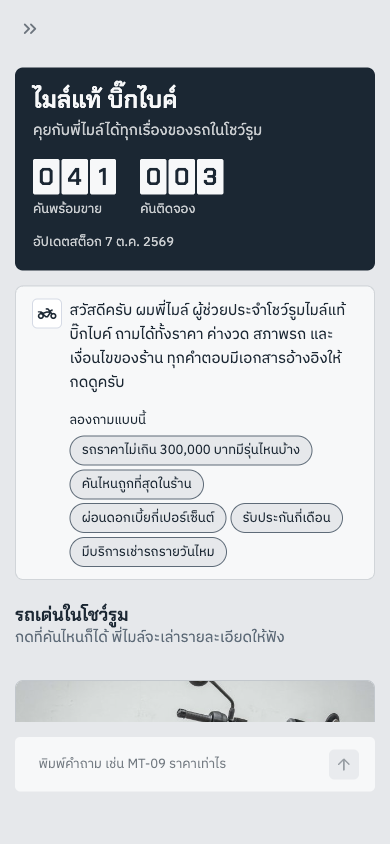
\includegraphics[width=0.38\textwidth]{img/08-mobile.png}}
\caption{หน้าแรกบนมือถือ (กว้าง 390px)}
\end{figure}
บนจอแคบ แถบหัว ปุ่มคำถาม และการ์ดรถเรียงซ้อนลงมาเป็นแถวเดียว ส่วน sidebar (ข้อมูลติดต่อและปุ่มล้างแชต) ซ่อนอยู่หลังปุ่ม \texttt{>>}

% ---------------- 5 ----------------
\section{ผลการทดสอบ}
\begin{itemize}
  \item \textbf{Retrieval} (\texttt{python rag.py} ไม่เรียก LLM): hit@5 = 25/26 = 96\% สำหรับคำถามที่ตอบได้
        ข้อที่พลาดคือถามด้วยรหัสสต็อก ``MT043'' ซึ่ง embedding จับรหัสได้ไม่ดี แต่ Gemini ยังตอบถูกจากตารางสต็อกที่ส่งไปทั้งตาราง
  \item \textbf{ทดสอบกับ Gemini จริง:} ราคา MT-09, ค่างวดแบบคำถามต่อเนื่อง, รถรหัส MT043, คันที่ถูกที่สุด และรถที่ติดจอง ตอบถูกทุกข้อพร้อมอ้างอิง
        คำถามที่ไม่มีคำตอบ (เช่น เช่ารถ) ตอบ ``ไม่พบข้อมูลในเอกสาร''
  \item \textbf{Threshold:} คะแนน e5 ของคำถามนอกเรื่องอยู่ที่ 0.80--0.87 ใกล้กับคำถามจริง threshold (0.78) จึงตัดเฉพาะคำถามที่ไม่เกี่ยวเลย
        ส่วนที่เหลือให้ prompt เป็นตัวปฏิเสธ
\end{itemize}

\section{วิธีใช้งานและ Deploy}
\begin{enumerate}
  \item รันบนเครื่อง: \texttt{pip install -r requirements.txt} แล้วใส่ \texttt{GEMINI\_API\_KEY} ใน \texttt{.streamlit/secrets.toml} (ไฟล์นี้อยู่ใน \texttt{.gitignore}) จากนั้น \texttt{streamlit run app.py}
  \item Deploy: สร้างแอปที่ share.streamlit.io จาก repository นี้ เลือก Python 3.12 และใส่ \texttt{GEMINI\_API\_KEY} ใน Secrets
  \item โหลดโมเดล embedding และสร้าง FAISS index ครั้งเดียวด้วย \texttt{@st.cache\_resource} ใช้ torch แบบ CPU เพื่อประหยัดพื้นที่และ RAM
\end{enumerate}

\end{document}
